\subsubsection{Schichtenarchitektur}
\label{sec:Kap-7.1.2.1}

\vspace{\baselineskip} %%% für Druck

\begin{figure}[h!]
	\centering
	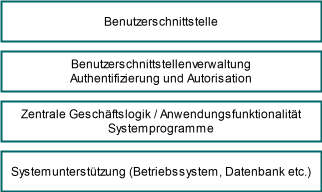
\includegraphics{Bilder/Kapitel-7/schichtenarchitektur_allgemein.pdf}
	\caption[Eine allgemeine Schichtenarchitektur]{Eine allgemeine Schichtenarchitektur, nach \cite[204]{som18}}
	\label{fig:schichtenarchitektur_allgemein}
\end{figure}

\vspace{\baselineskip} %%% für Druck

Abbildung~\ref{fig:schichtenarchitektur_allgemein} zeigt eine Schichtenarchitektur. Jede Schicht bildet einen logisch zusammenhängenden Zuständigkeitsbereich und setzt sich in der Regel aus mehreren Komponenten zusammen. In Systemen mit Benutzerinteraktion ist die oberste Schicht der Architektur die Benutzungsschnittstelle. Der Begriff Komponente im Zusammenhang mit Schichtenarchitektur benennt meist nicht das ganz „große“ Teilstück des Softwaresystems. Es handelt sich hier oft um die kleineren Einheiten, aus denen sich die großen Teilstücke zusammensetzen. Grundsätzlich abstrahiert das Modell der Schichtenarchitektur aber davon, was genau man in einem konkreten Softwareentwicklungsprojekt später als logische Einheit „Komponente“ 
\linebreak %%% für Druck
definiert.

Das grundsätzliche Prinzip bei einer Schichtenarchitektur ist, dass die Komponenten einer tieferliegenden Schicht die Dienstleister für die Komponenten der höheren Schichten sind, aber nicht umgekehrt. Das bedeutet, dass Komponenten in einer unteren Schicht für die Erbringung ihrer Funktionalität niemals auf die Funktionali\-täten von Komponenten einer höheren Schicht angewiesen sein dürfen. Abhängigkeiten einer Komponente kann es dann nur zu Komponenten unter ihr geben. Wenn dieses Prinzip eingehalten wird, kann es bei Veränderung oder Austausch einer bestimmten Komponente maximal Auswirkungen auf sie nutzende Komponenten in den darüber liegenden Schichten geben.

In einer sogenannten \textbf{strikten} Schichtenarchitektur dürfen Komponenten einer 
\linebreak %%% für Druck
Schicht nur Funktionalität von Komponenten der unmittelbar darunter liegenden Schicht verwenden. Das ist aber für viele Softwaresysteme nicht praktikabel und würde sich dort nur durch Codeduplizierung oder durch zusätzliche Komponenten, die rein für das „Durchleiten“ zuständig sind, realisieren lassen – beides widerspricht allgemeinen Entwurfsprinzipien. Daher werden Schichtenarchitekturen üblicherweise so eingesetzt, dass eine Komponente auch über mehrere Schichten hinweg auf Funktionalität einer in der Schichtenarchitektur unter ihr liegenden Komponente zugreifen kann.

Schichten sind lediglich logische Entwurfsgruppierungen von Komponenten des Softwaresystems. Sie werden bei der Implementierung üblicherweise nicht als ein eigenes „Konstrukt“ in den Programmcode übertragen. Im Programmcode direkt finden sich maximal die Komponenten (als Formen von Containerstrukturen wie zum Beispiel Packages in Java). Das zentrale Element im Programmcode sind die Klassen und diese sind aus Entwurfssicht gesehen die Bestandteile, aus denen sich die Komponenten zusammensetzen. Schichten bilden sich im Programmcode nur indirekt über die Aufruf-Abhängigkeiten der einzelnen Klassen untereinander ab.  

\begin{figure}[h!]
	\centering
	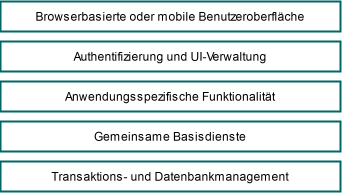
\includegraphics{Bilder/Kapitel-7/schichtenarchitektur_fuer_webbasierte_anwendungen.pdf}
	\caption[Eine Schichtenarchitektur für webbasierte Anwendungen]{Eine Schichtenarchitektur für webbasierte Anwendungen, nach \cite[108]{som20}}
	\label{fig:schichtenarchitektur_fuer_webbasierte_anwendungen}
\end{figure}

Eine Schichtenarchitektur muss nicht aus genau vier Schichten bestehen wie in \mbox{Abbildung}~\ref{fig:schichtenarchitektur_allgemein}. Die Anzahl der Schichten hängt vom konkret zu entwickelnden Software\-system und seinen geplanten Funktionalitäten ab. Für viele Anwendungs\-gebiete und Einsatzzwecke gibt es heute schon entsprechend angepasste detailliertere Schichtenarchitekturmodelle, die man gut als Ausgangspunkt für den Entwurf der eigenen Architektur verwenden kann. Abbildung~\ref{fig:schichtenarchitektur_fuer_webbasierte_anwendungen} zeigt eine verbreitete Schichtenarchitektur für webbasierte Softwareanwendungen. Bei \cite[108-113]{som20} finden Sie für diese Architektur eine detailliertere Beschreibung, welche Komponenten eines Softwaresystems man üblicherweise in welcher der Schichten platzieren würde, sowie die Anwendung dieser Architektur auf ein Fallbeispiel. Ein anderes Fallbeispiel mit vier Schichten zeigt \cite[214\psq]{som18}.